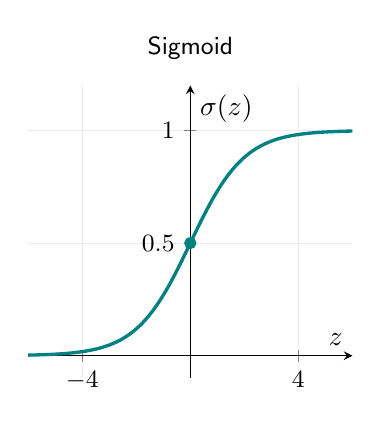
\begin{tikzpicture}
\begin{axis}[width=0.47\textwidth,height=53mm,axis lines=middle,
  xmin=-6,xmax=6,ymin=-0.1,ymax=1.2,xlabel={$z$},ylabel={$\sigma(z)$},
  xtick={-4,0,4},ytick={0.5,1},tick label style={font=\small},
  title={Sigmoid},title style={font=\small\sffamily},grid=major,grid style={gray!15}]
\addplot[Teal,very thick,domain=-6:6,samples=100]{1/(1+exp(-x))};
\addplot[only marks,mark=*,Teal] coordinates {(0,0.5)};
\end{axis}
\end{tikzpicture}\hfill
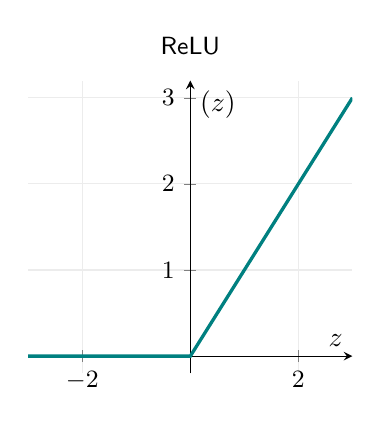
\begin{tikzpicture}
\begin{axis}[width=0.47\textwidth,height=53mm,axis lines=middle,
  xmin=-3,xmax=3,ymin=-0.2,ymax=3.2,xlabel={$z$},ylabel={$\ReLU(z)$},
  xtick={-2,0,2},ytick={1,2,3},tick label style={font=\small},
  title={ReLU},title style={font=\small\sffamily},grid=major,grid style={gray!15}]
\addplot[Teal,very thick] coordinates {(-3,0)(0,0)(3,3)};
\end{axis}
\end{tikzpicture}
